\documentclass{article}

\usepackage[a4paper, total={7in, 10in}]{geometry}

\usepackage{hyperref}
\usepackage{amsmath}
\usepackage{subcaption}
\usepackage{parskip}
\usepackage{graphicx}
\graphicspath{{../Results/Protected/}}

\title{AIMS Course 1: Data, Estimation and Inference}
\author{Jake Levi}
\date{October 2022}

\begin{document}
\maketitle
\section{Introduction} \label{section:intro}
We consider optimisation problems consisting of a decision variable $x$, which takes values in a set $\mathcal{X}$ (referred to as the domain of $x$), an objective function $f_0(x)$, inequality constraints $f_i(x)$ (for $i\in\{1, \hdots, m\}$), and equality constraints $h_i(x)$ (for $i\in\{1, \hdots, p\}$), which can be expressed in` the following form:
\begin{equation}
\begin{aligned}
    \underset{x \in \mathcal{X}}{\text{Minimise}} \quad & f_0(x) \\
    \text{Subject to} \quad & f_i(x) \le 0 \quad i\in\{1, \hdots, m\} \\
    & h_i(x) = 0 \quad i\in\{1, \hdots, p\}
\end{aligned} \label{eq:optimisation problem}
\end{equation}
We refer to the set of values of $x\in\mathcal{X}$ which satisfy the equality and inequality constraints as the feasible set, which is denoted by $\mathcal{F}$:
\begin{equation}
    \mathcal{F} = \{ x\in\mathcal{X}: (\forall i\in\{1, \hdots, m\}) \quad f_i(x) \le 0 \quad \text{and} \quad (\forall i\in\{1, \hdots, p\}) \quad h_i(x) = 0 \}
\end{equation}
The limit of the smallest value of $f_0(x)$ for any value of $x$ in the feasible set $\mathcal{F}$ is referred to as the optimal cost, and denoted by $p^*$:
\begin{equation}
    p^* = \underset{x\in\mathcal{F}}{\inf}\left[f_0(x)\right]
\end{equation}
When solving an optimisation problem in the form described by equation \ref{eq:optimisation problem}, it is useful to introduce the Lagrangian function \cite{boyd2004convex} (intuition for the form of the Lagrangian function is provided in appendix \ref{appendix:why lagrangian}), which is a function of the decision variable $x\in\mathcal{X}$, and also the variables $\lambda \in \mathbb{R}^m $ and $\nu\in\mathbb{R}^p$, which are referred to as the Lagrange multipliers for the inequality and equality constraints respectively:
\begin{equation}
    \mathcal{L}(x, \lambda, \nu) = f_0(x) + \sum_{i=1}^{m}[\lambda_i f_i(x)] + \sum_{i=1}^{p}[\nu_i h_i(x)] \label{eq:Lagrangian}
\end{equation}
The limit of the smallest value of the Lagrangian function for any value of $x$ in its domain $\mathcal{X}$ (not only in the feasible set $\mathcal{F}$) as a function of the Lagrange multipliers $\lambda$ and $\nu$ is referred to as the Lagrange dual function $g$:
\begin{align}
    g(\lambda, \nu) &= \underset{x\in\mathcal{X}}{\inf}\left[\mathcal{L}(x, \lambda, \nu)\right] \label{eq:dual function} \\
    &= \underset{x\in\mathcal{X}}{\inf}\left[f_0(x) + \sum_{i=1}^{m}[\lambda_i f_i(x)] + \sum_{i=1}^{p}[\nu_i h_i(x)]\right]
\end{align}
The dual function is concave with respect to $\lambda$ and $\nu$, which is equivalent to the following statements:
\begin{align}
    (\forall\lambda^{(1)},\lambda^{(2)}\in\mathbb{R}^m)(\forall\alpha\in[0, 1]) \quad g(\alpha\lambda^{(1)} + (1 - \alpha)\lambda^{(2)}, \nu) &\ge \alpha g(\lambda^{(1)}, \nu) + (1 - \alpha) g(\lambda^{(2)}, \nu) \label{eq:dual concave lambda} \\
    (\forall\nu^{(1)},\nu^{(2)}\in\mathbb{R}^p)(\forall\alpha\in[0, 1]) \quad g(\lambda, \alpha\nu^{(1)} + (1 - \alpha)\nu^{(2)}) &\ge \alpha g(\lambda, \nu^{(1)}) + (1 - \alpha) g(\lambda, \nu^{(2)})\label{eq:dual concave nu}
\end{align}
Both of these statements can be easily proved. We start by proving equation \ref{eq:dual concave lambda}, for which it is useful to define the variable $x^*\in\bar{\mathcal{X}}$ (where $\bar{\mathcal{X}}$ denotes the closure of the set $\mathcal{X}$) which satisfies the following equation, given $\alpha$, $\lambda^{(1)}$, $\lambda^{(2)}$, and $\nu$:
\begin{align}
    \underset{x\in\mathcal{X}}{\inf}\left[\mathcal{L}(x, \alpha\lambda^{(1)} + (1 - \alpha)\lambda^{(2)}, \nu)\right] &= \mathcal{L}(x^*, \alpha\lambda^{(1)} + (1 - \alpha)\lambda^{(2)}, \nu) \\
    \Rightarrow & \begin{cases}
        \underset{x\in\mathcal{X}}{\inf}\left[\mathcal{L}(x, \lambda^{(1)}, \nu)\right] \le \mathcal{L}(x^*, \lambda^{(1)}, \nu) \\
        \underset{x\in\mathcal{X}}{\inf}\left[\mathcal{L}(x, \lambda^{(2)}, \nu)\right] \le \mathcal{L}(x^*, \lambda^{(2)}, \nu)
    \end{cases} \\
    \Rightarrow \alpha \underset{x\in\mathcal{X}}{\inf}\left[\mathcal{L}(x, \lambda^{(1)}, \nu)\right] + (1 - \alpha) \underset{x\in\mathcal{X}}{\inf}\left[\mathcal{L}(x, \lambda^{(2)}, \nu)\right] &\le \alpha\mathcal{L}(x^*, \lambda^{(1)}, \nu) + (1 - \alpha)\mathcal{L}(x^*, \lambda^{(2)}, \nu) \\
    &= \mathcal{L}(x^*, \alpha\lambda^{(1)} + (1 - \alpha)\lambda^{(2)}, \nu) \label{eq:follows from Lagrangian} \\
    &= \underset{x\in\mathcal{X}}{\inf}\left[\mathcal{L}(x, \alpha\lambda^{(1)} + (1 - \alpha)\lambda^{(2)}, \nu)\right] \\
    \Rightarrow (\forall\lambda^{(1)},\lambda^{(2)}\in\mathbb{R}^m)(\forall\alpha\in[0, 1]) \quad \alpha g(\lambda^{(1)}, \nu) + (1 - \alpha) g(\lambda^{(2)}, \nu) &\le g(\alpha\lambda^{(1)} + (1 - \alpha)\lambda^{(2)}, \nu) \label{eq:follows from dual}
\end{align}
Where (\ref{eq:follows from Lagrangian}) follows from the definition of the Lagrangian function $\mathcal{L}$ in equation \ref{eq:Lagrangian} and the fact that $\alpha + (1 - \alpha) = 1$, and (\ref{eq:follows from dual}) follows from the definition of the Lagrangian dual function $g$ in equation \ref{eq:dual function}. The proof that the dual Lagrangian function is concave with respect to $\nu$ (equation \ref{eq:dual concave nu}) follows using similar reasoning.

We also note that for any $\lambda \ge 0$ (where $\ge$ is understood to apply element-wise to each element of $\lambda$) and for any $\nu$, the Lagrangian dual function $g(\lambda, \nu)$ is a lower bound for the optimal cost $p^*$. To prove this, it is useful to note that for any feasible point $\tilde{x}\in\mathcal{F}$ (which necessarily satisfies $f_i(x) \le 0$ for all $i\in\{1, \hdots, m\}$ and $h_i(x) = 0$ for all $i\in\{1, \hdots, p\}$), and for any $\lambda\ge 0$ and any $\nu$, the following inequality holds:
\begin{align}
    (\forall \tilde{x} \in \mathcal{F}, \lambda \ge 0, \nu) \quad 0 &\ge \sum_{i=1}^{m}[\lambda_i f_i(\tilde{x})] + \sum_{i=1}^{p}[\nu_i h_i(\tilde{x})] \\
    \Rightarrow (\forall \tilde{x} \in \mathcal{F}, \lambda \ge 0, \nu) \quad f_0(\tilde{x}) &\ge f_0(\tilde{x}) + \sum_{i=1}^{m}[\lambda_i f_i(\tilde{x})] + \sum_{i=1}^{p}[\nu_i h_i(\tilde{x})] \\
    &= \mathcal{L}(\tilde{x}, \lambda, \nu) \\
    &\ge \underset{x\in\mathcal{X}}{\inf}\left[\mathcal{L}(x, \lambda, \nu)\right] \\
    &= g(\lambda, \nu)
\end{align}
Since this is true for any feasible $\tilde{x}$, it is also true for the value of $\tilde{x} \in \mathcal{F}$ which minimises the objective function, $f_0(x)$:
\begin{align}
    (\forall \tilde{x} \in \mathcal{F}, \lambda \ge 0, \nu) \quad g(\lambda, \nu) &\le f_0(\tilde{x}) \\
    \Rightarrow (\forall \lambda \ge 0, \nu) \quad g(\lambda, \nu) &\le \underset{x\in\mathcal{F}}{\inf}\left[f_0(x)\right] \\
    &= p^*
\end{align}
The limit of the greatest value of $g(\lambda, \nu)$ for any $\lambda \ge 0$ and $\nu$ is the best lower bound on $p^*$, and is referred to as the dual optimal cost, denoted by $d^*$:
\begin{align}
    d^* &= \underset{\lambda \ge 0, \nu}{\sup}\left[g(\lambda, \nu)\right] \\
    &= \underset{\lambda \ge 0, \nu}{\sup}\left[\underset{x\in\mathcal{X}}{\inf}\left[\mathcal{L}(x, \lambda, \nu)\right]\right] \\
    & \le p^*
\end{align}
Therefore we have that the dual optimal cost $d^*$ is always less than or equal to the primal optimal cost, $p^*$. An interesting symmetry exists between the optimal cost $p^*$ (also referred to as the primal optimal cost) and the dual optimal cost, $d^*$. To see this, we start by noting that the Lagrangian function $\mathcal{L}(x, \lambda, \nu)$ is unbounded above (and below) with respect to $\lambda$ and $\nu $ unless $x$ is in the feasible set $\mathcal{F}$, in which case the Lagrangian function is bounded above by the objective function, $f_0(x)$:
\begin{align}
    \underset{\lambda \ge 0, \nu}{\sup}\left[ \mathcal{L}(x, \lambda, \nu) \right] &= \begin{cases}
        f_0(x) & x \in \mathcal{F} \\
        \infty & \text{otherwise}
    \end{cases} \\
    \Rightarrow \underset{x\in\mathcal{X}}{\inf}\left[\underset{\lambda \ge 0, \nu}{\sup}\left[\mathcal{L}(x, \lambda, \nu)\right]\right] &= \underset{x\in\mathcal{F}}{\inf}\left[f_0(x)\right] \\
    &= p^* \\
    \Rightarrow \underset{\lambda \ge 0, \nu}{\sup}\left[\underset{x\in\mathcal{X}}{\inf}\left[\mathcal{L}(x, \lambda, \nu)\right]\right] &\le \underset{x\in\mathcal{X}}{\inf}\left[\underset{\lambda \ge 0, \nu}{\sup}\left[\mathcal{L}(x, \lambda, \nu)\right]\right]
\end{align}
This latter inequality is a special case of the Max–min inequality, and in the context of optimisation, it is known as the principle of weak duality. In cases where equality holds, and the dual optimal cost is equal to the primal optimal cost, $d^* = p^*$, this is known as strong duality.

\begin{figure}[pht]
    \centering
    \subfloat[
        \centering Training and ground truth data
        \label{fig:data}
    ]{
        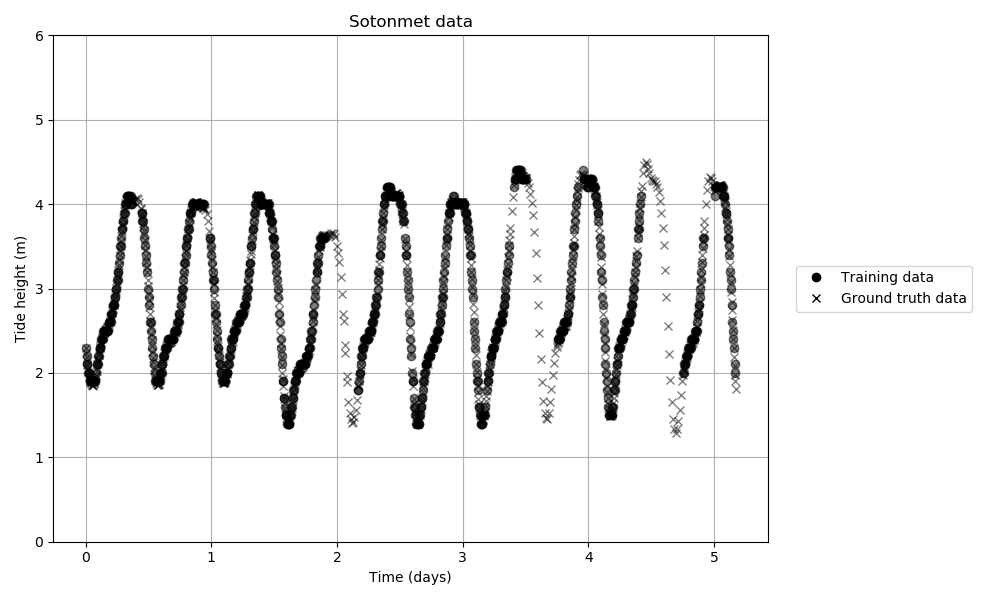
\includegraphics[width=0.45\textwidth]{Sotonmet_data.png}
    }
    \subfloat[
        \centering Independent GP predictions
        \label{fig:ind_pres}
    ]{
        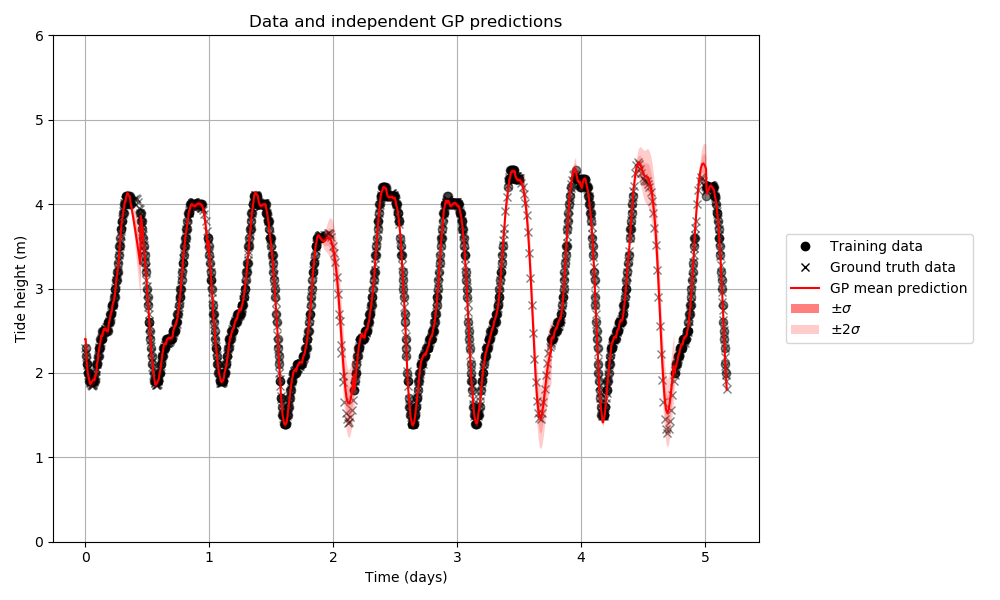
\includegraphics[width=0.45\textwidth]{Data_and_independent_GP_predictions.png}
    }
    \caption{The Sotonmet dataset}
    \label{fig:sotonmet}
\end{figure}

\section{Results}
\subsection{Squared Exponential Kernels}
We start off by considering GPs with constant mean function and squared exponential kernel, whose mean and kernel functions are related to the hyperparameters $c$, $k$, and $\lambda$ as follows ($\sigma$ is also considered to be a hyperparameter, although it is not explicitly part of the mean or kernel functions):
% Equation: constant mean and squared exponential kernel function
\begin{align}
\mu(x) &= c \\
K_{\mathrm{sqe}}(x, x') &= k \exp\left( -\left( \frac{x - x'}{\lambda} \right)^2 \right)
\end{align}
Initially we consider two GPs denoted by sqe\_1 and sqe\_2, whose hyperparameter values are described in table \ref{table:sqe hyperparameters}. Samples from the prior distributions of sqe\_1 and sqe\_1 are shown in figures \ref{fig:prior_sqe_1} and \ref{fig:prior_sqe_2}, which show that the prior distribution of sqe\_1 looks subjectively like a much more plausible explanation for the data. The predictive distributions of these GPs are shown in figures \ref{fig:pred_dist_sqe_1} and \ref{fig:pred_dist_sqe_2}, which show that, although sqe\_1 produced a \emph{prior} distribution which looks like a more plausible explanation for the training data, sqe\_2 produces a \emph{predictive} distribution which looks like a much better fit to the training data. Furthermore, the predictive distribution of sqe\_1 is "confidently wrong" (the mean is far away from the ground truth labels and with high certainty/low standard deviation) in regions containing ground truth labels but no training data, which would be a very undesirable property of a machine learning prediction model in a safety-critical context. Samples from the predictive distribution of both GPs are shown in figures \ref{fig:pred_samples_sqe_1} and \ref{fig:pred_samples_sqe_2}, which show that neither GP produces samples that reflect the data distribution particularly well.

The evaluation of GPs sqe\_1 and sqe\_2 according to the metrics RMSE (square root of the mean-squared-error between labels and the GP's predictive mean), LML, and log predictive likelihood (LPL, which is just the logarithm of equation \ref{eq:conditional distribution} given the expression for a multivariate Gaussian probability density function \cite{bishop2006pattern}), is summarised in table \ref{table:metrics}. Note that although sqe\_1 has a very low RMSE evaluated on the training data, it has an RMSE which is $30\times$ higher when evaluated on the ground truth data, which is to say that sqe\_1 overfits the training data very badly, which is reflected in its relatively bad LML and LPLs. sqe\_2 has worse RMSE on the training data than the sqe\_1, but better RMSE on the ground truth data, which is to say that sqe\_2 generalises better to unseen data (although it does so with low confidence/high uncertainty, as seen in sqe\_2's predictive samples in figure \ref{fig:pred_samples_sqe_2}), and this is reflected in the better LML and LPLs of sqe\_2.

As mentioned in section \ref{section:intro}, the LML can be used as an objective function to optimise the hyperparameters of a GP. Starting with sqe\_2 (because this GP has greater LML than sqe\_1), the parameters of this GP can be optimised using the L-BFGS-B algorithm \cite{wright1999numerical}, leading to a GP referred to as sqe\_opt, whose hyperparameter values are described in table \ref{table:sqe hyperparameters}, and whose evaluation metrics are described in table \ref{table:metrics}. Remarkably, sqe\_opt has worse RMSE on \emph{training} data than sqe\_1, but better RMSE on \emph{unseen} ground truth data. This implies that optimising RMSE on training data (which is often performed in machine learning) is not always a good approach, because an improvement in the RMSE on training data might lead to decreased predictive performance on unseen data (which is generally of greater importance in machine learning), and that where possible, a better approach might be to optimise LML instead. The sensitivity of the LML of sqe\_opt to its hyperparameters is shown in figure \ref{fig:sqe sensitivity}, which shows that sqe\_opt is very sensitive to large values of $\lambda$ and small values of $\sigma$. The predictive distribution of sqe\_opt is shown in figure \ref{fig:pred_samples_sqe_opt}.

We start off by considering GPs with constant mean function and squared exponential kernel, whose mean and kernel functions are related to the hyperparameters $c$, $k$, and $\lambda$ as follows ($\sigma$ is also considered to be a hyperparameter, although it is not explicitly part of the mean or kernel functions):
% Equation: constant mean and squared exponential kernel function
\begin{align}
\mu(x) &= c \\
K_{\mathrm{sqe}}(x, x') &= k \exp\left( -\left( \frac{x - x'}{\lambda} \right)^2 \right)
\end{align}
Initially we consider two GPs denoted by sqe\_1 and sqe\_2, whose hyperparameter values are described in table \ref{table:sqe hyperparameters}. Samples from the prior distributions of sqe\_1 and sqe\_1 are shown in figures \ref{fig:prior_sqe_1} and \ref{fig:prior_sqe_2}, which show that the prior distribution of sqe\_1 looks subjectively like a much more plausible explanation for the data. The predictive distributions of these GPs are shown in figures \ref{fig:pred_dist_sqe_1} and \ref{fig:pred_dist_sqe_2}, which show that, although sqe\_1 produced a \emph{prior} distribution which looks like a more plausible explanation for the training data, sqe\_2 produces a \emph{predictive} distribution which looks like a much better fit to the training data. Furthermore, the predictive distribution of sqe\_1 is "confidently wrong" (the mean is far away from the ground truth labels and with high certainty/low standard deviation) in regions containing ground truth labels but no training data, which would be a very undesirable property of a machine learning prediction model in a safety-critical context. Samples from the predictive distribution of both GPs are shown in figures \ref{fig:pred_samples_sqe_1} and \ref{fig:pred_samples_sqe_2}, which show that neither GP produces samples that reflect the data distribution particularly well.

The evaluation of GPs sqe\_1 and sqe\_2 according to the metrics RMSE (square root of the mean-squared-error between labels and the GP's predictive mean), LML, and log predictive likelihood (LPL, which is just the logarithm of equation \ref{eq:conditional distribution} given the expression for a multivariate Gaussian probability density function \cite{bishop2006pattern}), is summarised in table \ref{table:metrics}. Note that although sqe\_1 has a very low RMSE evaluated on the training data, it has an RMSE which is $30\times$ higher when evaluated on the ground truth data, which is to say that sqe\_1 overfits the training data very badly, which is reflected in its relatively bad LML and LPLs. sqe\_2 has worse RMSE on the training data than the sqe\_1, but better RMSE on the ground truth data, which is to say that sqe\_2 generalises better to unseen data (although it does so with low confidence/high uncertainty, as seen in sqe\_2's predictive samples in figure \ref{fig:pred_samples_sqe_2}), and this is reflected in the better LML and LPLs of sqe\_2.

As mentioned in section \ref{section:intro}, the LML can be used as an objective function to optimise the hyperparameters of a GP. Starting with sqe\_2 (because this GP has greater LML than sqe\_1), the parameters of this GP can be optimised using the L-BFGS-B algorithm \cite{wright1999numerical}, leading to a GP referred to as sqe\_opt, whose hyperparameter values are described in table \ref{table:sqe hyperparameters}, and whose evaluation metrics are described in table \ref{table:metrics}. Remarkably, sqe\_opt has worse RMSE on \emph{training} data than sqe\_1, but better RMSE on \emph{unseen} ground truth data. This implies that optimising RMSE on training data (which is often performed in machine learning) is not always a good approach, because an improvement in the RMSE on training data might lead to decreased predictive performance on unseen data (which is generally of greater importance in machine learning), and that where possible, a better approach might be to optimise LML instead. The sensitivity of the LML of sqe\_opt to its hyperparameters is shown in figure \ref{fig:sqe sensitivity}, which shows that sqe\_opt is very sensitive to large values of $\lambda$ and small values of $\sigma$. The predictive distribution of sqe\_opt is shown in figure \ref{fig:pred_samples_sqe_opt}.

We start off by considering GPs with constant mean function and squared exponential kernel, whose mean and kernel functions are related to the hyperparameters $c$, $k$, and $\lambda$ as follows ($\sigma$ is also considered to be a hyperparameter, although it is not explicitly part of the mean or kernel functions):
% Equation: constant mean and squared exponential kernel function
\begin{align}
\mu(x) &= c \\
K_{\mathrm{sqe}}(x, x') &= k \exp\left( -\left( \frac{x - x'}{\lambda} \right)^2 \right)
\end{align}
Initially we consider two GPs denoted by sqe\_1 and sqe\_2, whose hyperparameter values are described in table \ref{table:sqe hyperparameters}. Samples from the prior distributions of sqe\_1 and sqe\_1 are shown in figures \ref{fig:prior_sqe_1} and \ref{fig:prior_sqe_2}, which show that the prior distribution of sqe\_1 looks subjectively like a much more plausible explanation for the data. The predictive distributions of these GPs are shown in figures \ref{fig:pred_dist_sqe_1} and \ref{fig:pred_dist_sqe_2}, which show that, although sqe\_1 produced a \emph{prior} distribution which looks like a more plausible explanation for the training data, sqe\_2 produces a \emph{predictive} distribution which looks like a much better fit to the training data. Furthermore, the predictive distribution of sqe\_1 is "confidently wrong" (the mean is far away from the ground truth labels and with high certainty/low standard deviation) in regions containing ground truth labels but no training data, which would be a very undesirable property of a machine learning prediction model in a safety-critical context. Samples from the predictive distribution of both GPs are shown in figures \ref{fig:pred_samples_sqe_1} and \ref{fig:pred_samples_sqe_2}, which show that neither GP produces samples that reflect the data distribution particularly well.

The evaluation of GPs sqe\_1 and sqe\_2 according to the metrics RMSE (square root of the mean-squared-error between labels and the GP's predictive mean), LML, and log predictive likelihood (LPL, which is just the logarithm of equation \ref{eq:conditional distribution} given the expression for a multivariate Gaussian probability density function \cite{bishop2006pattern}), is summarised in table \ref{table:metrics}. Note that although sqe\_1 has a very low RMSE evaluated on the training data, it has an RMSE which is $30\times$ higher when evaluated on the ground truth data, which is to say that sqe\_1 overfits the training data very badly, which is reflected in its relatively bad LML and LPLs. sqe\_2 has worse RMSE on the training data than the sqe\_1, but better RMSE on the ground truth data, which is to say that sqe\_2 generalises better to unseen data (although it does so with low confidence/high uncertainty, as seen in sqe\_2's predictive samples in figure \ref{fig:pred_samples_sqe_2}), and this is reflected in the better LML and LPLs of sqe\_2.

As mentioned in section \ref{section:intro}, the LML can be used as an objective function to optimise the hyperparameters of a GP. Starting with sqe\_2 (because this GP has greater LML than sqe\_1), the parameters of this GP can be optimised using the L-BFGS-B algorithm \cite{wright1999numerical}, leading to a GP referred to as sqe\_opt, whose hyperparameter values are described in table \ref{table:sqe hyperparameters}, and whose evaluation metrics are described in table \ref{table:metrics}. Remarkably, sqe\_opt has worse RMSE on \emph{training} data than sqe\_1, but better RMSE on \emph{unseen} ground truth data. This implies that optimising RMSE on training data (which is often performed in machine learning) is not always a good approach, because an improvement in the RMSE on training data might lead to decreased predictive performance on unseen data (which is generally of greater importance in machine learning), and that where possible, a better approach might be to optimise LML instead. The sensitivity of the LML of sqe\_opt to its hyperparameters is shown in figure \ref{fig:sqe sensitivity}, which shows that sqe\_opt is very sensitive to large values of $\lambda$ and small values of $\sigma$. The predictive distribution of sqe\_opt is shown in figure \ref{fig:pred_samples_sqe_opt}.

\begin{figure}
    \centering
    \begin{subfigure}{0.45\textwidth}
        \centering
        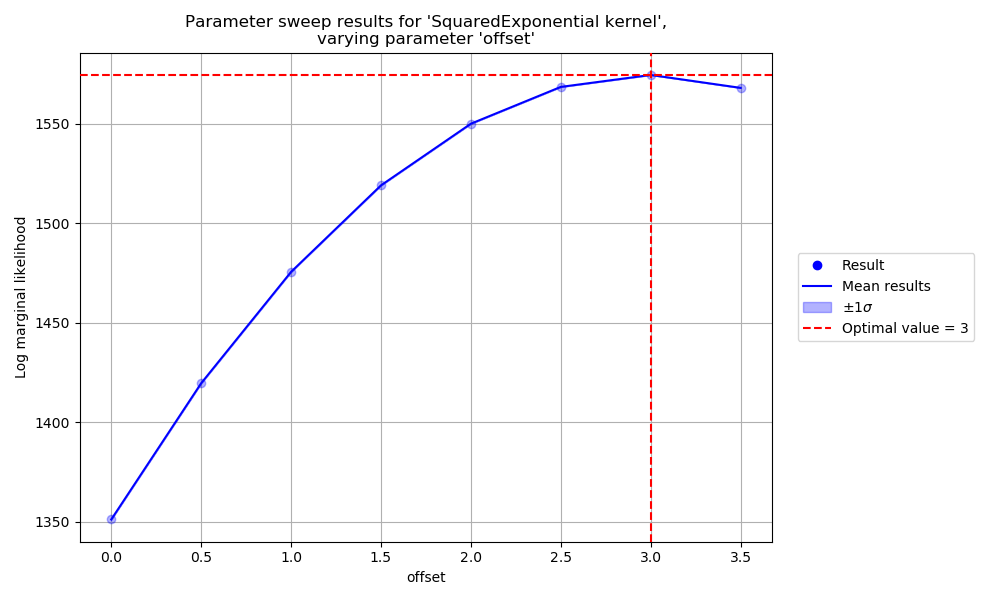
\includegraphics[width=\textwidth]{param_sweep/SquaredExponential/Parameter_sweep_results_for__SquaredExponential_kernel_,_varying_parameter__offset_.png}
        \caption{$c$}
        \label{fig:sqe offset}
    \end{subfigure}
    \begin{subfigure}{0.45\textwidth}
        \centering
        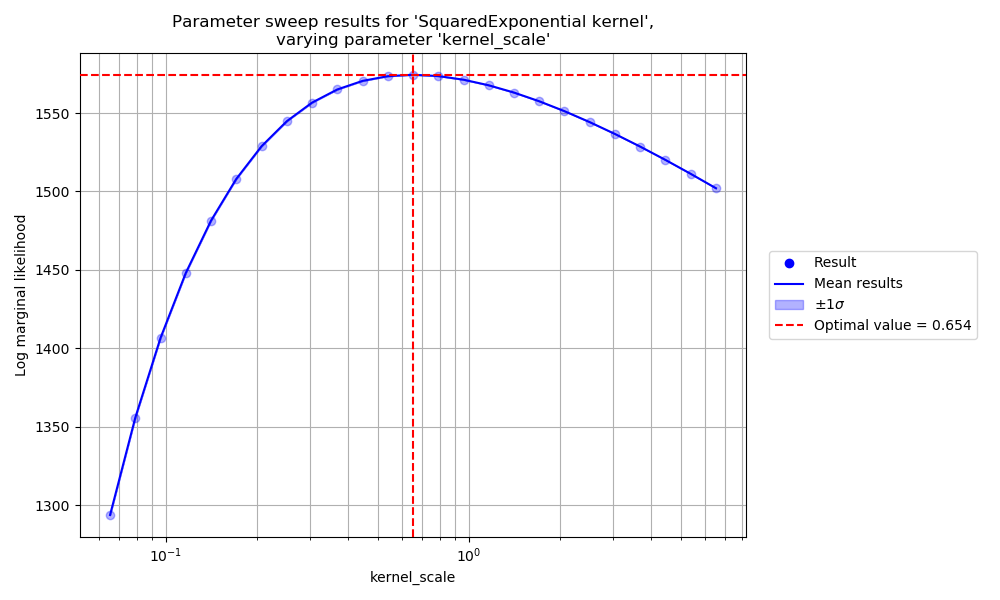
\includegraphics[width=\textwidth]{param_sweep/SquaredExponential/Parameter_sweep_results_for__SquaredExponential_kernel_,_varying_parameter__kernel_scale_.png}
        \caption{$k$}
        \label{fig:sqe kernel scale}
    \end{subfigure}
    \newline
    \begin{subfigure}{0.45\textwidth}
        \centering
        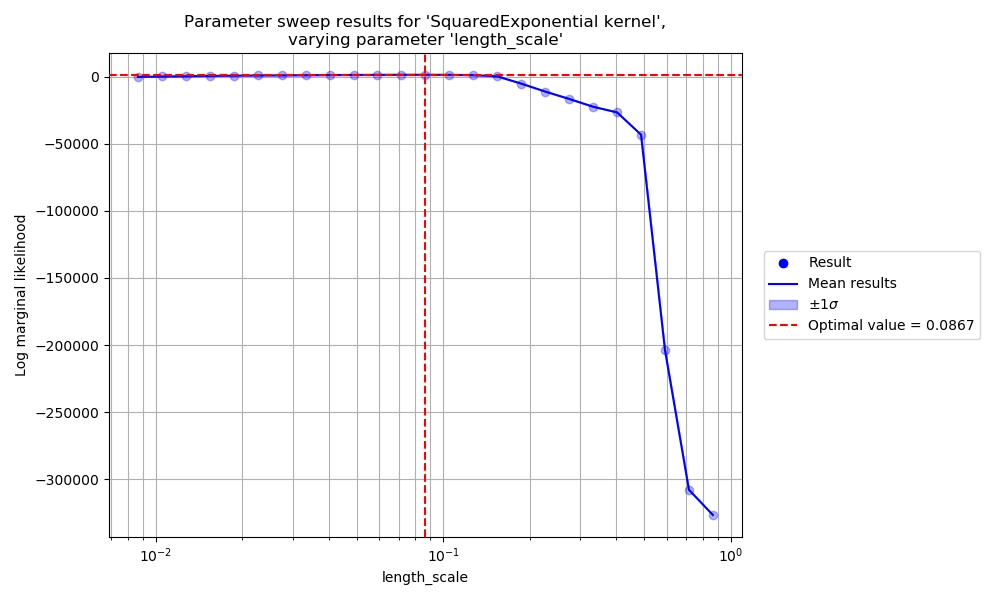
\includegraphics[width=\textwidth]{param_sweep/SquaredExponential/Parameter_sweep_results_for__SquaredExponential_kernel_,_varying_parameter__length_scale_.png}
        \caption{$\lambda$}
        \label{fig:sqe length scale}
    \end{subfigure}
    \begin{subfigure}{0.45\textwidth}
        \centering
        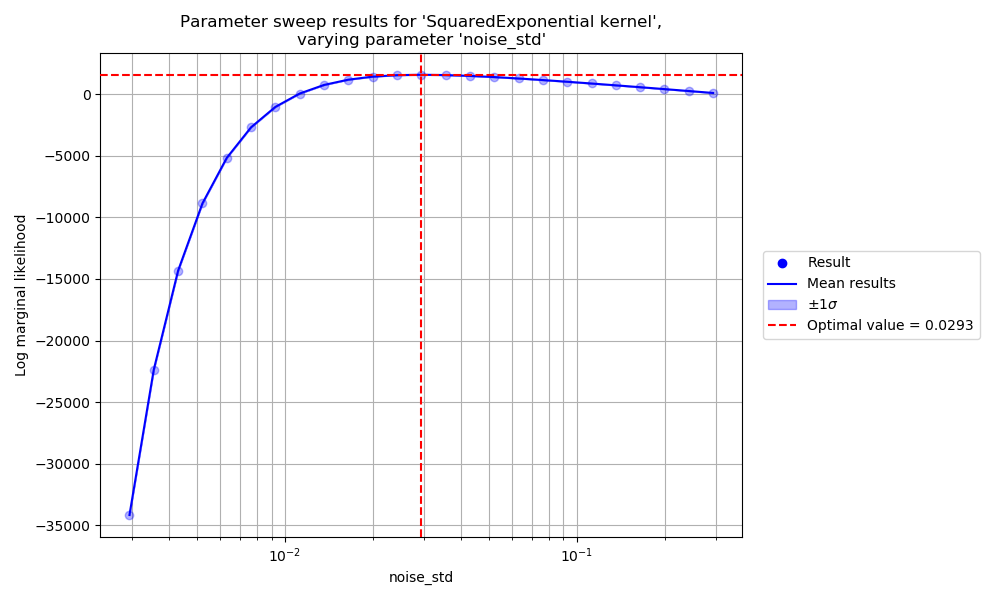
\includegraphics[width=\textwidth]{param_sweep/SquaredExponential/Parameter_sweep_results_for__SquaredExponential_kernel_,_varying_parameter__noise_std_.png}
        \caption{$\sigma$}
        \label{fig:sqe noise}
    \end{subfigure}

    \caption{Sensitivity of the LML of sqe\_opt to its hyperparameters}
    \label{fig:sqe sensitivity}
\end{figure}

\begin{figure}[pht]
    \centering
    \begin{subfigure}{0.45\textwidth}
        \centering
        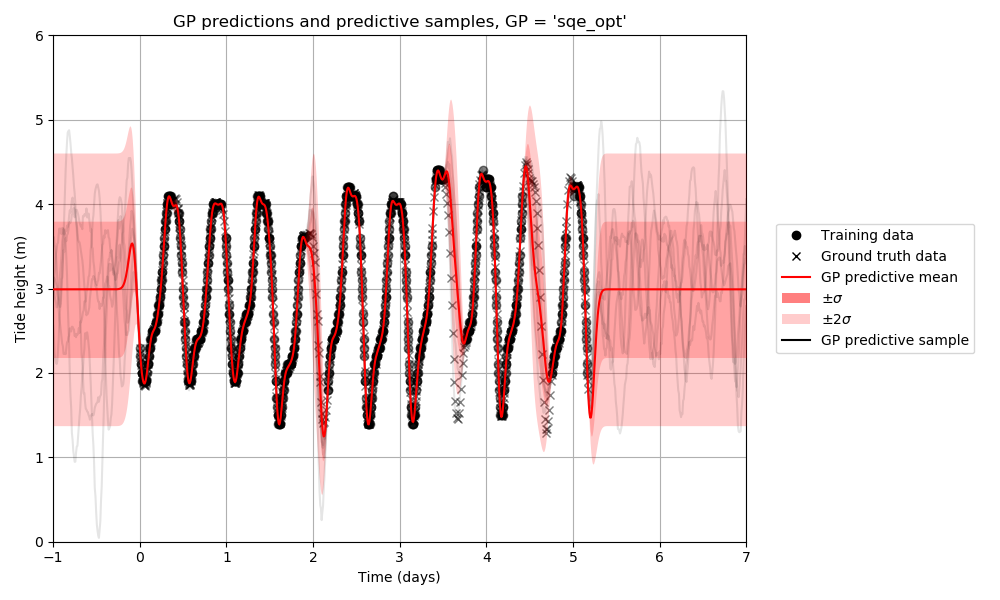
\includegraphics[width=\textwidth]{GP_predictions_and_predictive_samples,_GP____sqe_opt_.png}
        \caption{sqe\_opt}
        \label{fig:pred_samples_sqe_opt}
    \end{subfigure}
    \begin{subfigure}{0.45\textwidth}
        \centering
        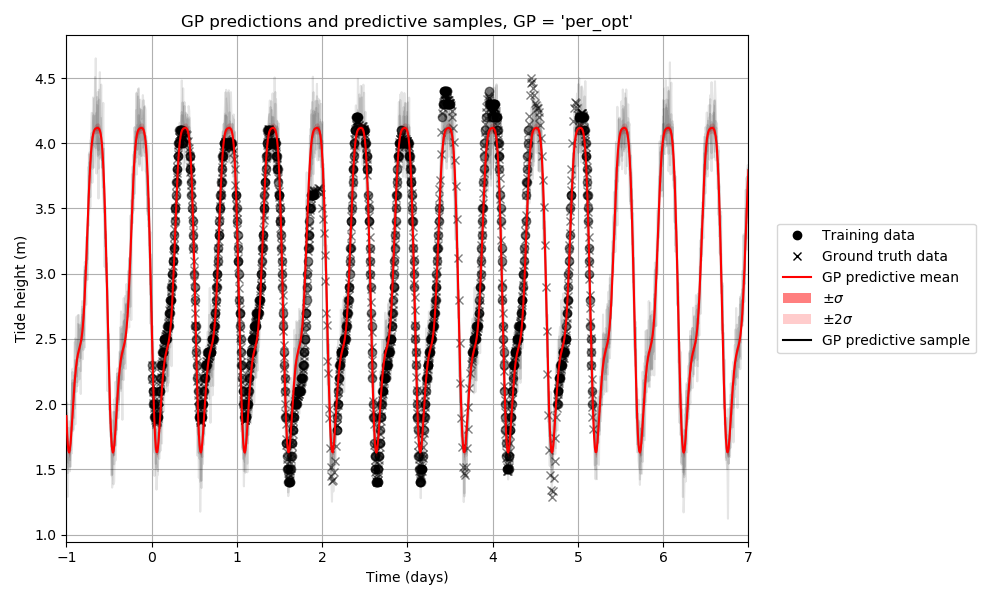
\includegraphics[width=\textwidth]{GP_predictions_and_predictive_samples,_GP____per_opt_.png}
        \caption{per\_opt}
        \label{fig:pred_samples_per_opt}
    \end{subfigure}
    \newline
    \begin{subfigure}{0.45\textwidth}
        \centering
        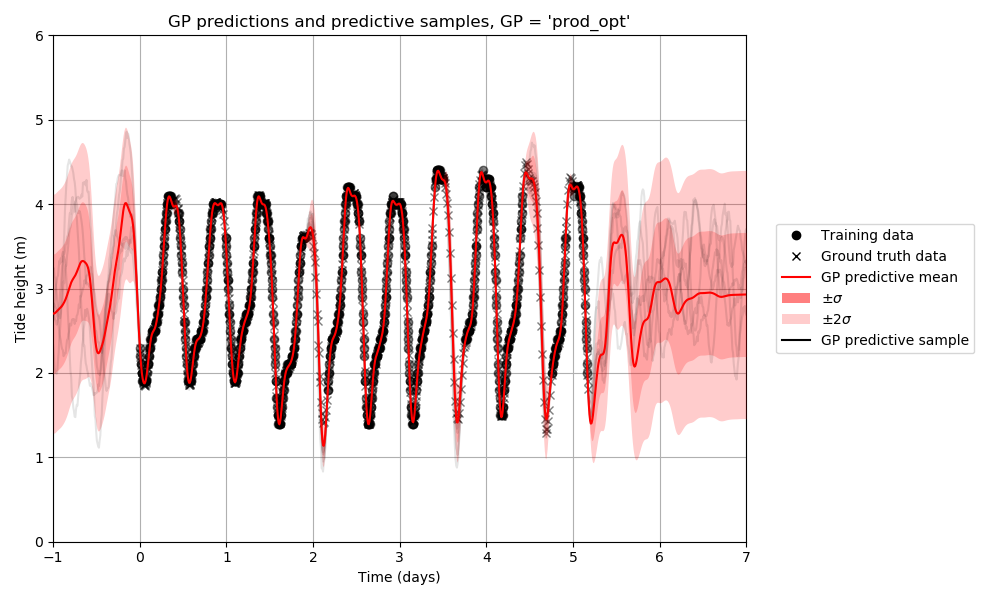
\includegraphics[width=\textwidth]{GP_predictions_and_predictive_samples,_GP____prod_opt_.png}
        \caption{prod\_opt}
        \label{fig:pred_samples_prod_opt}
    \end{subfigure}
    \begin{subfigure}{0.45\textwidth}
        \centering
        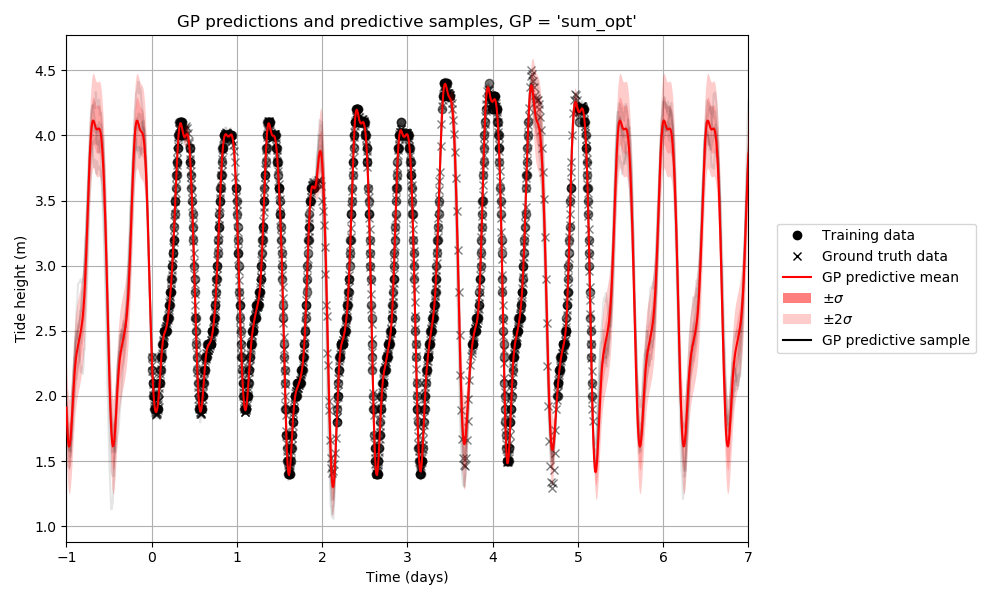
\includegraphics[width=\textwidth]{GP_predictions_and_predictive_samples,_GP____sum_opt_.png}
        \caption{sum\_opt}
        \label{fig:pred_samples_sum_opt}
    \end{subfigure}

    \caption{Predictive distributions of GPs with different kernel functions and optimised hyperparameters}
    \label{fig:opt}
\end{figure}

\pagebreak
\subsection{Epistemic and aleatoric uncertainty}
To quote Alex Kendall and Yarin Gal in \cite{kendall2017uncertainties}:

\begin{quote}
    There are two major types of uncertainty one can model. Aleatoric uncertainty captures noise inherent in the observations. On the other hand, epistemic uncertainty accounts for uncertainty in the model - uncertainty which can be explained away given enough data.
\end{quote}

We can model the performance of a GP in the presence of epistemic or aleatoric uncertainty by either removing a subsection of the data or by artificially adding noise to a subsection of the data respectively. In the case of sqe\_opt (which was optimised to have high LML), the results of two such experiments are shown in figure \ref{fig:uncertainty}.

Although this GP performs well in the presence of epistemic uncertainty, reverting to a larger predictive standard deviation when far from the vicinity of any training data, we see that this GP does not perform well in the presence of aleatoric uncertainty, making confidently wrong predictions (predictions which are far away from the ground truth labels and with high certainty/low standard deviation) in the vicinity of training data which has a high degree of noise.

We can understand this behaviour by looking at the expression for the predictive variance of a GP in equation \ref{eq:conditional variance}, which depends only on the input locations of the training data and predictions, and not on the labels of the training data. Of course, the predictive variance of sqe\_opt considered here depends indirectly on the training labels, as a result of its hyperparameters having been optimised with respect to the LML of the training data, however this model has no capacity to increase its predictive uncertainty in the presence of unseen noisy training labels.

This could be a very undesirable property for the model to have in a safety-critical prediction context, for example if one of the input sensors failed and started producing very noisy measurements, we would not want the model to produce wildly incorrect predictions with a high degree of certainty, rather we would prefer the model to increase its predictive uncertainty to fit the noise in the newly observed data. One possible solution to this problem would be to model the observation noise (which does directly affect the predictive uncertainty of a GP) using a second GP, which predicts observation noise as a function of the same input data as the original GP, and conditions on the estimated noise of the training data, however we leave this as a direction for future work.

To quote Alex Kendall and Yarin Gal in \cite{kendall2017uncertainties}:

\begin{quote}
    There are two major types of uncertainty one can model. Aleatoric uncertainty captures noise inherent in the observations. On the other hand, epistemic uncertainty accounts for uncertainty in the model - uncertainty which can be explained away given enough data.
\end{quote}

We can model the performance of a GP in the presence of epistemic or aleatoric uncertainty by either removing a subsection of the data or by artificially adding noise to a subsection of the data respectively. In the case of sqe\_opt (which was optimised to have high LML), the results of two such experiments are shown in figure \ref{fig:uncertainty}.

Although this GP performs well in the presence of epistemic uncertainty, reverting to a larger predictive standard deviation when far from the vicinity of any training data, we see that this GP does not perform well in the presence of aleatoric uncertainty, making confidently wrong predictions (predictions which are far away from the ground truth labels and with high certainty/low standard deviation) in the vicinity of training data which has a high degree of noise.

We can understand this behaviour by looking at the expression for the predictive variance of a GP in equation \ref{eq:conditional variance}, which depends only on the input locations of the training data and predictions, and not on the labels of the training data. Of course, the predictive variance of sqe\_opt considered here depends indirectly on the training labels, as a result of its hyperparameters having been optimised with respect to the LML of the training data, however this model has no capacity to increase its predictive uncertainty in the presence of unseen noisy training labels.

This could be a very undesirable property for the model to have in a safety-critical prediction context, for example if one of the input sensors failed and started producing very noisy measurements, we would not want the model to produce wildly incorrect predictions with a high degree of certainty, rather we would prefer the model to increase its predictive uncertainty to fit the noise in the newly observed data. One possible solution to this problem would be to model the observation noise (which does directly affect the predictive uncertainty of a GP) using a second GP, which predicts observation noise as a function of the same input data as the original GP, and conditions on the estimated noise of the training data, however we leave this as a direction for future work.

\bibliographystyle{plain}
\bibliography{references}
\appendix
\section{Motivation for maximising the log marginal likelihood}\label{appendix:why_lml}
\end{document}
